\pagebreak
\section{Multiparameter device optimizer}
\label{sec:device_optimizer}
Related YouTube videos:

\begin{figure}[H]
\begin{tabular}{ c l }

\includegraphics[width=0.05\textwidth]{./images/youtube.png}
&
\href{https://www.youtube.com/watch?v=L5o0ogp67vE}{Optimizing the layer structure of a Perovskite solar cell}
\end{tabular}
\end{figure}

\begin{figure}[H]
\begin{tabular}{ c l }


\includegraphics[width=0.05\textwidth]{./images/youtube.png}

&
\href{https://www.youtube.com/watch?v=sBhCg9lWjZ8 }{Optimizing an OPV device for maximum photon harvesting.}

\end{tabular}
\end{figure}

\begin{figure}[H]
\begin{tabular}{ c l }


\includegraphics[width=0.05\textwidth]{./images/youtube.png}

&
\href{https://www.youtube.com/watch?v=60RVozhJqFY  }{Searching for the optimum layer structure in an organic solar cell.}

\end{tabular}
\end{figure}

Very often when optimizing a device an engineer or scientists will be want to know what the optimum structure of a device is. For example a perovskite solar cell is made up of multiple layers, but what is the optimum thickness of each layer? If the perovskite layer is made really thick then lots of light will be absorbed but the down side of this is that it will take longer for charge carriers to escape the device so recombination will be high.  Conversely if the layer is made really thin very few carriers will have a chance to recombine as they will not spend long in the device but the downside is that not many photons will be absorbed in the first place as the layer is thin.  If one then also considers that light will reflect multiple times of interfaces in the device setting up standing wave pattens, this will further complicate the optimization problem as one will need to optimize not only the thickness of the perovskite layer but also the thicknesses of all other layers at the same time. To solve this multi-parameter optimization problem one can use the \emph{Fast optimizer} within the scan window.

\subsection{Using the multi parameter optimizer}
In the new simulation window under the sub-topic \emph{Scripting and fitting} there are several examples of multi-parameter optimizers:

\begin{itemize}
  \item Electrical layer optimizer: This will vary the layer thickness of two active layers of an organic solar cell simulation and plot the PEC/FF/Voc as a function of these layer thicknesses.
  \item Optical layer optimizer (perovskite): This will vary the thickness of two layers in a perovskite solar cell and plot the current generated by each layer within the device.
  \item Optical layer optimizer (OPV): This will vary the thickness of two layers in a perovskite solar cell and plot the current generated by each layer within the device.
\end{itemize}

In this text we will be using the \emph{Optical layer optimizer (perovskite)}, if you open this simulation and navigate to the scan window, you will see a scan already set up called \emph{optimizer}. If you open it you will get a window shown in figure \ref{fig:device_optimizer}. This scan window looks just like the scan windows described in the previous section, however the key difference is that the \emph{Fast optimizer} button is depressed. When this button is depressed scan results are not written to disk, instead the key simulation parameters are tabulated and saved to disk at the end of the simulation.  Notice that in this example we are varying the thickness (dy) of the Perovskite layer between 300nm and 500 nm in steps of 10 nm and the thickness (dy) TiO2 layer from 100 nm to 300 nm also in steps of 10 nm. Try running the simulation, the using windows explorer navigate to your simulation directory, then open the folder called \emph{optimize} and in there you will find a \emph{csv} file called \emph{optimizer\_output.csv}. If you open this with Excel or LibreOffice, it will look like figure \ref{fig:device_optimizer_output}.

\begin{figure}
\centering
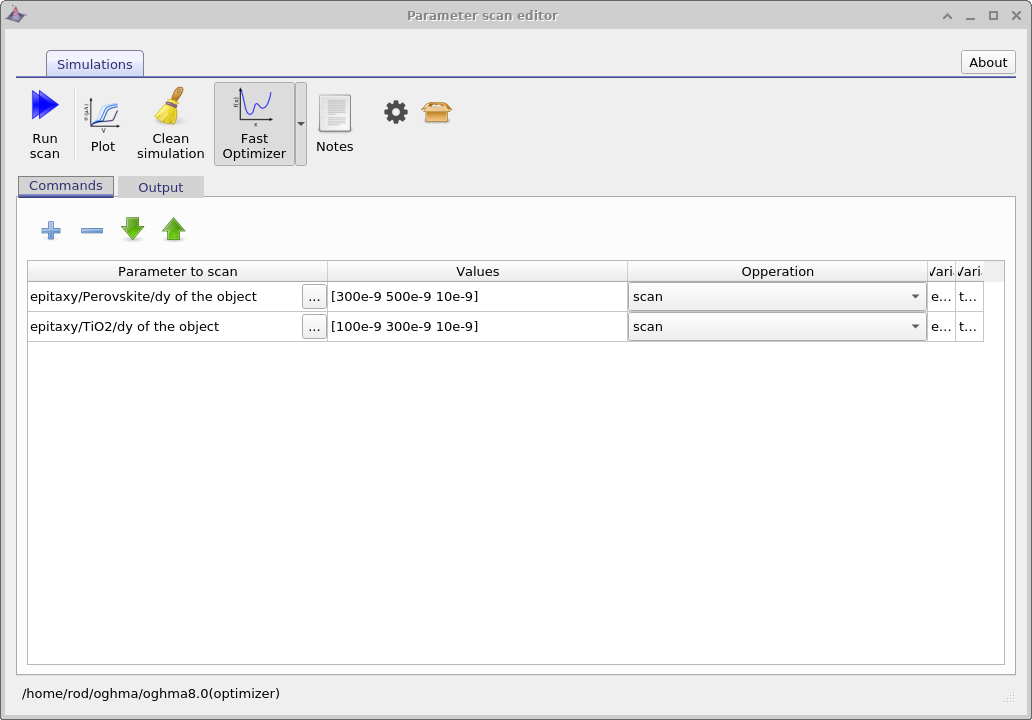
\includegraphics[width=0.6\linewidth,height=0.5\linewidth]{./images/scan_optimizer.png}
\caption{The scan window with the optimizer button depressed ready to run a device layer optimization.}
\label{fig:device_optimizer}
\end{figure}

If you examine figure \ref{fig:device_optimizer_output} carefully you can see the first two columns are labelled epitaxy.layer2.dy and epitaxy.layer1.dy . These are the layer thicknesses we decided to change in the scan window.  For every subsequent layer in the device there are two columns, labelled layerX/light\_frac\_photon\_generation and layerX/J. These refer to the fraction of the light absorbed with in the layer and the maximum current this layer would produce if all the light absorbed within the layer were turned into current. Clearly if light is absorbed within the active layer it has a good chance of being turned into current, however if light is absorbed within the back metallic contact  then there is little chance of that light being turned into electrical current. If you use the sorting tools included within Excel/LibreOffice you can figure out which device structures produce the most current.

\begin{figure}
\centering
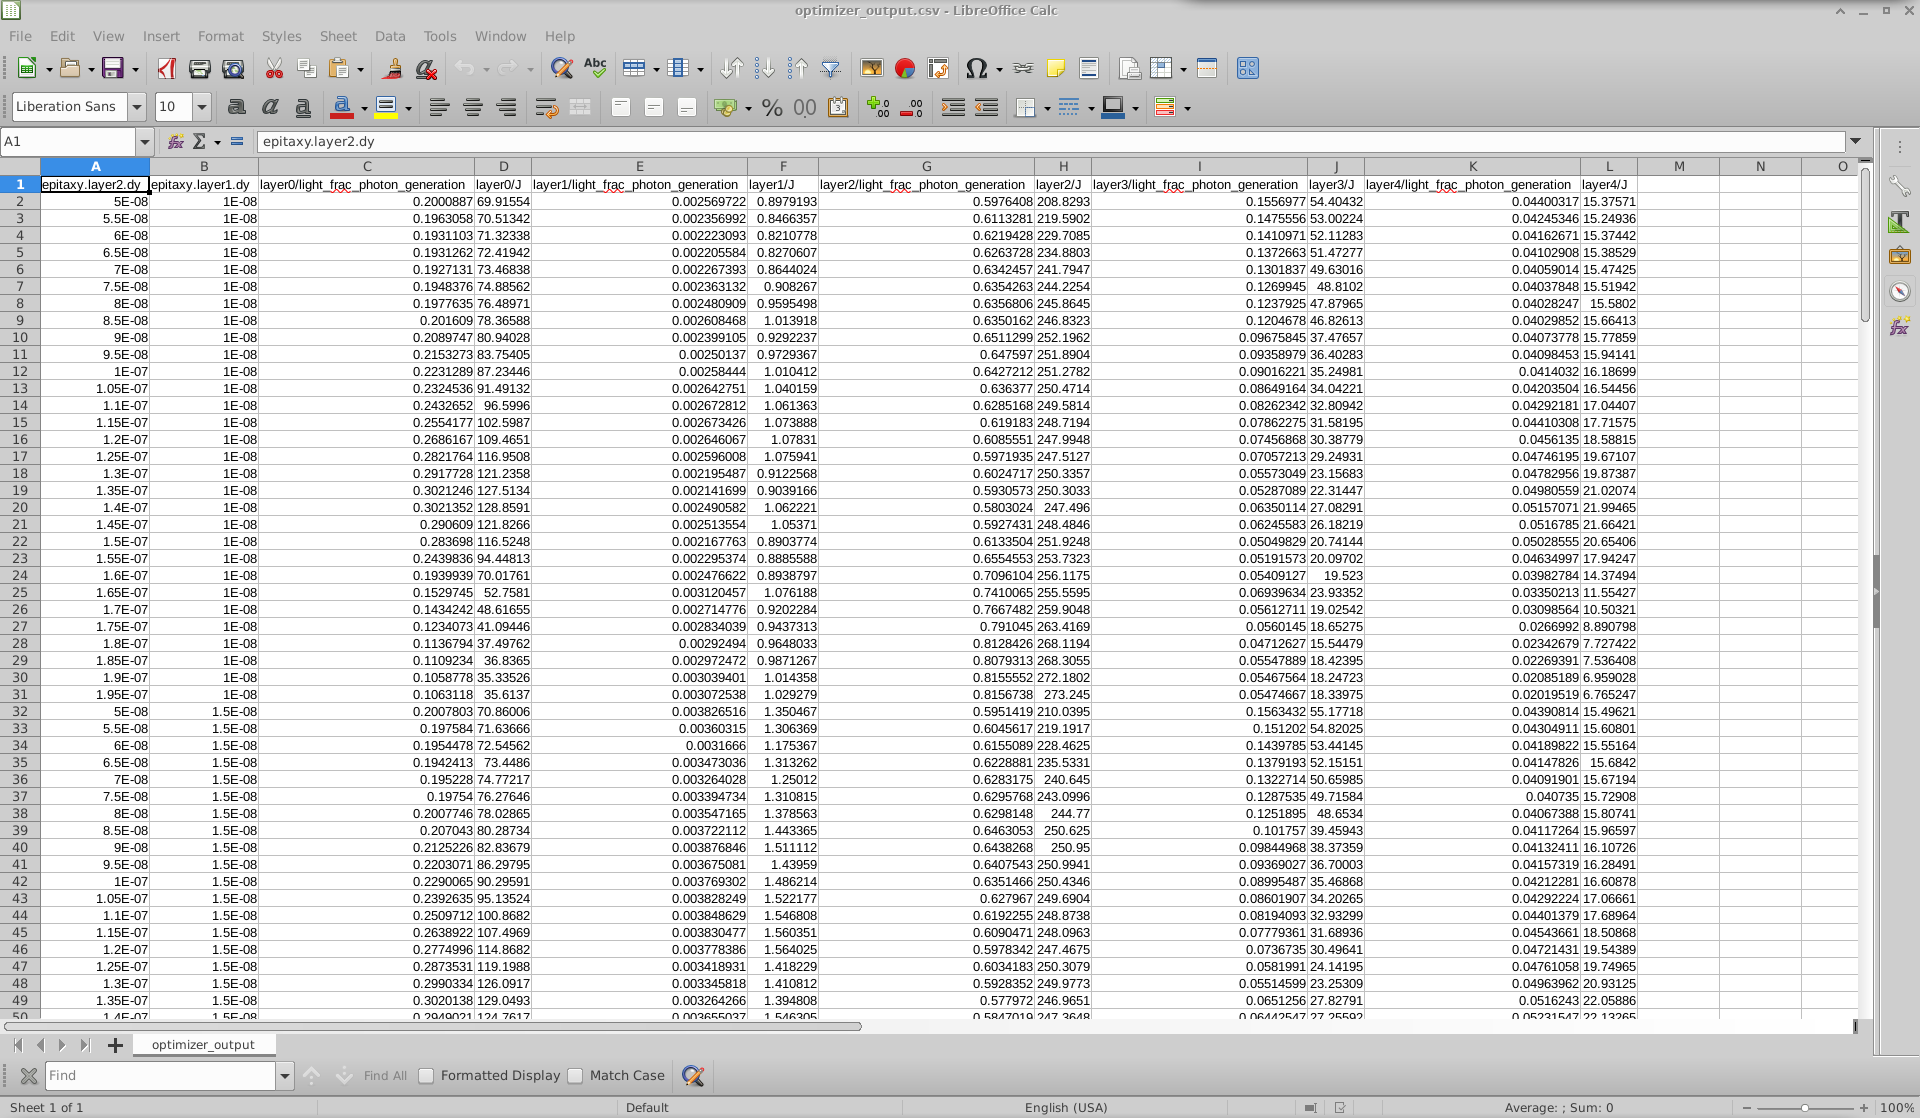
\includegraphics[width=\linewidth]{./images/scan_optimizer_output.png}
\caption{The file your simulation directory/optimizer/optimizer\_output.csv} opened in LibreOffice (You can use Excel).
\label{fig:device_optimizer_output}
\end{figure}
\vfill
